\subsection{Near-extremal principal-mode enhancement}
\label{sec:principal20261014}

We next hold the asymptotic incident amplitude and
$y=p/\kappa\ne0$ fixed while approaching extremal rotation, with $m>0$.
The frequency then approaches $\omega_*=m/(2M)$.
This path probes concentration of the incident-normalized field in the Kerr
throat.  We define
\begin{equation}
\sigma=\frac{r_+-r_-}{M},\qquad
\widehat\chi_n=M^{2n-2}\frac{T_n^{(1)}}{T^{(0)}}.
\label{eq:principal-parameters}
\end{equation}
Since $M\kappa=\sigma/[4(1+\sigma/2)]$, the leading powers in $\sigma$
and $M\kappa$ agree.  In the following connection formulas we set $M=1$.
The normalization is unit ingoing horizon amplitude for $R_{\rm in}$ and
unit outgoing infinity amplitude for $R_{\rm up}$.

\subsubsection{The throat equation and its two branches}

Let $X=(r-r_+)/\sigma$.  The exact relations
$\Delta=\sigma^2X(X+1)$ and $(r_+^2+a^2)p=\sigma y/2$ give
\begin{equation}
K=\sigma\left(\frac y2+2r_+\omega X+\sigma\omega X^2\right).
\end{equation}
At fixed $X,y$ the leading radial equation is
\begin{equation}
\frac{d}{dX}\left[X(X+1)\frac{df}{dX}\right]
+\left[\frac{(mX+y/2)^2}{X(X+1)}-\lambda_*\right]f=0,
\label{eq:principal-near-ode}
\end{equation}
where $\lambda_*=A_{\ell m}(m/2)-3m^2/4$ in our angular convention.
In the overlap region the indicial equation gives
\begin{align}
h(h-1)+m^2-\lambda_*&=0,\nonumber\\
h&=\frac12+\sqrt{\frac14+A_{\ell m}(m/2)-\frac{7m^2}{4}}.
\label{eq:principal-weight}
\end{align}
The two branches are $X^{h-1}$ and $X^{-h}$.
The principal class has $h=1/2+i\beta$, $\beta>0$, so both branches have
the same $X^{-1/2}$ amplitude envelope.  The real-weight class has distinct
real exponents.  This classification follows from the radial equation
\cite{BredbergKerrCFT2010}.

The horizon-ingoing solution is
\begin{align}
f_y(X)={}&X^{-iy/2}(1+X)^{i(y/2-m)}\nonumber\\
&\times{}_2F_1(h-im,1-h-im;1-iy;-X).
\label{eq:principal-near-solution}
\end{align}
Continuation to large $X$ yields $f_y\sim c_+X^{h-1}+c_-X^{-h}$, with
\begin{align}
c_+&=\frac{\Gamma(1-iy)\Gamma(2h-1)}
{\Gamma(h-im)\Gamma[h-i(y-m)]},\nonumber\\
c_-&=\frac{\Gamma(1-iy)\Gamma(1-2h)}
{\Gamma(1-h-im)\Gamma[1-h-i(y-m)]}.
\label{eq:principal-near-connection}
\end{align}

\subsubsection{Connection to asymptotically flat radiation}

At extremality set $u=r-1$.  The critical-frequency outer equation becomes
\begin{equation}
u^2R''+2uR'+[m^2(1+u/2)^2-\lambda_*]R=0.
\label{eq:principal-outer-ode}
\end{equation}
Setting $\Psi=uR$ and $z=-imu$ gives the Whittaker equation
\begin{equation}
\frac{d^2\Psi}{dz^2}
+\left[-\frac14+\frac{im}{z}+
\frac{1/4-(h-1/2)^2}{z^2}\right]\Psi=0.
\end{equation}
The solutions normalized to $u^{h-1}$ and $u^{-h}$ are
\begin{align}
R_+(u)&=(-im)^{-h}u^{-1}M_{im,h-1/2}(-imu),\nonumber\\
R_-(u)&=(-im)^{h-1}u^{-1}M_{im,1/2-h}(-imu).
\end{align}
Their incoming amplitudes are
\begin{align}
U_+&=\frac{\Gamma(2h)}{\Gamma(h-im)}(-im)^{-h-im},\nonumber\\
U_-&=\frac{\Gamma(2-2h)}{\Gamma(1-h-im)}(-im)^{h-1-im}.
\label{eq:principal-outer-connection}
\end{align}
These coefficients share a unit-modulus phase determined by the additive
constant in $r_*$.  We use the principal branch of $\log(-im)$ consistently.
The near hypergeometric and outer Whittaker representations implement the
leading near-extremal analytic connection.  MST supplies the full-frequency
series and connection structure\cite{MST1996}; its renormalized angular
momentum $\nu$ and the throat index $h$ label the respective representations.

In the overlap region $u\simeq\sigma X$, matching gives
\begin{align}
B^{\rm inc}&\sim c_+U_+\sigma^{1-h}+c_-U_-\sigma^h\nonumber\\
&=\sigma^{1/2}{\cal D}(\theta),\qquad\theta=\beta\ln\sigma,\nonumber\\
{\cal D}(\theta)&=c_+U_+e^{-i\theta}+c_-U_-e^{i\theta}.
\label{eq:principal-incidence}
\end{align}
Thus fixed-incident normalization yields
\begin{equation}
|R_H^{(0)}|^2\sim\frac{\sigma^{-1}}{|{\cal D}(\theta)|^2}.
\label{eq:principal-density}
\end{equation}
The near-critical horizon flux carries an additional factor $p\propto\sigma$.
Consequently the linear absorption is finite and log-phase dependent, with
$T^{(0)}\sim y/[m|{\cal D}|^2]$ in $M=1$ units.

\subsubsection{The nonlinear source integral and the envelope law}

Choose near solutions $\psi_+\sim X^{h-1}$ and $\psi_-\sim X^{-h}$.
The outgoing Whittaker solution $u^{-1}W_{im,h-1/2}(-imu)$ has overlap
coefficients
\begin{align}
g_+&=\frac{\Gamma(1-2h)}{\Gamma(1-h-im)}(-im)^h,\nonumber\\
g_-&=\frac{\Gamma(2h-1)}{\Gamma(h-im)}(-im)^{1-h}.
\end{align}
Its near-zone form is $R_{\rm up}\sim\sigma^{-1/2}\gamma_\theta$, where
\begin{equation}
\gamma_\theta=g_+e^{i\theta}\psi_++g_-e^{-i\theta}\psi_-.
\end{equation}
The constant near Wronskian and its physical counterpart are
\begin{align}
w_\theta&=X(X+1)(f_y\gamma_\theta'-\gamma_\theta f_y'),\nonumber\\
W&\sim\sigma^{1/2}w_\theta.
\end{align}
The covariant source weight at the limiting horizon is
$C_H^{(n)}=C^{(0,n)}_{\ell\ell m}+C^{(2,n)}_{\ell\ell m}$.
Since $dr=\sigma\,dX$, the Green projection gives the finite leading
unit-horizon coefficient
\begin{equation}
{\cal A}_n(\theta)=-\frac{C_H^{(n)}}{w_\theta}
\int_0^\infty\gamma_\theta|f_y|^{2n}f_y\,dX.
\label{eq:principal-source-integral}
\end{equation}
At $X=0$ the amplitude envelope is bounded.  At large $X$ the integrand
envelope is $X^{-n-1}$, so the integral converges for every positive integer
$n$.  The factors $\sigma^{-1/2}$ from $R_{\rm up}$, $\sigma$ from $dr$,
and $\sigma^{-1/2}$ from $1/W$ cancel.  The remaining real power in the
fixed-incident response therefore comes from $|B^{\rm inc}|^{-2n}$:
\begin{align}
\widehat\chi_n&=\sigma^{-n}{\cal F}_n(y,\theta)+o(\sigma^{-n}),\nonumber\\
{\cal F}_n(y,\theta)&=\frac{2\operatorname{Re}{\cal A}_n(\theta)}
{|{\cal D}(\theta)|^{2n}}.
\label{eq:principal-law}
\end{align}
The expansion applies on compact parameter sets where the matching
denominators stay bounded away from zero.  At a zero of
$\operatorname{Re}{\cal A}_n$, the next term controls the flux response.
Transforming $\theta\mapsto\theta+\pi$ changes the signs of $\gamma,w$ and
$\mathcal D$ while preserving $\mathcal A_n$ and $|\mathcal D|$.
The leading coefficient hence has logarithmic period $\pi/\beta$.
The envelope power is $-n$, and the two-branch interference determines its
log-periodic modulation.

For reproducible coefficient evaluation, write $\gamma=a_\theta f_y+
b_\theta f_y^*$.  The horizon current gives
$|c_+|^2-|c_-|^2=-y/(2\beta)$ and $w_\theta=iyb_\theta$.
Let $G_+=g_+e^{i\theta}$, $G_-=g_-e^{-i\theta}$ and
$d_c=|c_+|^2-|c_-|^2$.  Then
\begin{align}
a_\theta&=(G_+c_+^*-G_-c_-^*)/d_c,\nonumber\\
b_\theta&=(-G_+c_-+G_-c_+)/d_c,\nonumber\\
{\cal A}_n&=\frac{iC_H^{(n)}}{y}
\left(\frac{a_\theta}{b_\theta}I_n^{\rm osc}+I_n^{\rm abs}\right),\nonumber\\
I_n^{\rm osc}&=\int_0^\infty f_y^2|f_y|^{2n}\,dX,\qquad
I_n^{\rm abs}=\int_0^\infty|f_y|^{2n+2}\,dX.
\label{eq:principal-integral-evaluation}
\end{align}
Equations~\eqref{eq:principal-near-connection}--\eqref{eq:principal-integral-evaluation}
specify the leading prediction with zero fitted parameters.

\subsubsection{Real weights and the perturbative domain}

For a real nondegenerate $h>1/2$, the dominant incident connection has
$B^{\rm inc}\sim c_+U_+\sigma^{1-h}$ and the incident-normalized near
field scales as $\sigma^{h-1}$.  The projected Green integrand in the
overlap region scales as $X^{2n(h-1)-1}$.
For $1/2<h<1$ the upper integral converges and the throat contribution
has power $\sigma^{2n(h-1)}$.  For $h>1$, the matching upper limit
$X\sim\sigma^{-1}$ supplies $\sigma^{-2n(h-1)}$; the resulting
order-unity contribution is determined by the full outer matching.
At $h=1$ the upper integral has logarithmic behavior.
This convergence criterion specifies when a local throat power controls
the complete observable.  The real-weight channel $(1,1)$ has
$h=1.1706059743$ and belongs to the upper-limit-sensitive class.

Define $g_n=\epsilon_n/M^{2n-2}$ and the dimensionless complex horizon
response $\widehat\rho_n$, with
$\widehat\chi_n=2\operatorname{Re}\widehat\rho_n$.
The leading field correction has
$\widehat\rho_n\sim\sigma^{-n}{\cal A}_n/|{\cal D}|^{2n}$.
The relative horizon-field and flux corrections obey, respectively,
\begin{equation}
\begin{split}
|g_n|\,|{\cal A}_{\rm in}|^{2n}|\widehat\rho_n|&\ll1,\\
|g_n|\,|{\cal A}_{\rm in}|^{2n}|\widehat\chi_n|&\ll1.
\end{split}
\label{eq:principal-validity}
\end{equation}
The field condition controls both the horizon amplitude and its phase.
On principal-mode intervals with a bounded nonzero typical coefficient,
the expansion parameter scales as
$|g_n||{\cal A}_{\rm in}|^{2n}(M\kappa)^{-n}$.
This identifies the shrinking weak-coupling domain near extremality.

\subsubsection{Expanded numerical verification}

\begin{table}[t]
\caption{Critical scalar angular eigenvalues and principal weights at
$a/M=1$, $M\omega=m/2$, with $h=1/2+i\beta$.}
\label{tab:principal-weights20261014}
\begin{ruledtabular}\begin{tabular}{ccc}
$(\ell,m)$ & $A_{\ell m}$ & $\beta$\\
$(2,2)$ & 5.8551625746 & 0.9459584692 \\
$(3,3)$ & 11.7447939547 & 1.9378354020 \\
$(4,4)$ & 19.6267345276 & 2.8501342902 \\
\end{tabular}\end{ruledtabular}\end{table}
\begin{table*}[t]
\caption{Parameter-free leading matching at $a/M=0.999999$.
The three middle columns give relative differences between the spectral
response and the matched prediction, in percent.  $\delta_N$ is the maximum
paired spectral response change across the three spins and three interaction
orders at fixed $q=3072$; $\delta_q$ is the corresponding change at fixed
$N=448$ under $q=1536\to3072$.}
\label{tab:principal-verification20261014}
\begin{ruledtabular}\begin{tabular}{ccccccc}
$(\ell,m)$ & $y$ & $n=1$ (\%) & $n=2$ (\%) & $n=3$ (\%) & $\delta_N$ & $\delta_q$\\
$(2,2)$ & -0.5 & 1.925 & 2.403 & 2.422 & $4.13\times10^{-9}$ & $6.71\times10^{-7}$\\
$(2,2)$ & 0.5 & 0.825 & 0.964 & 0.894 & $8.43\times10^{-11}$ & $3.82\times10^{-6}$\\
$(2,2)$ & 1 & 0.782 & 0.717 & 0.581 & $1.26\times10^{-11}$ & $5.39\times10^{-5}$\\
$(3,3)$ & -0.5 & 0.202 & 0.516 & 0.834 & $6.55\times10^{-9}$ & $1.24\times10^{-6}$\\
$(3,3)$ & 0.5 & 0.111 & 0.307 & 0.506 & $1.26\times10^{-10}$ & $1.02\times10^{-5}$\\
$(3,3)$ & 1 & 0.053 & 0.178 & 0.305 & $1.41\times10^{-11}$ & $7.81\times10^{-5}$\\
$(4,4)$ & -0.5 & 0.042 & 0.343 & 0.665 & $1.21\times10^{-9}$ & $1.16\times10^{-6}$\\
$(4,4)$ & 0.5 & 0.066 & 0.294 & 0.537 & $1.56\times10^{-10}$ & $1.21\times10^{-5}$\\
$(4,4)$ & 1 & 0.030 & 0.182 & 0.379 & $1.46\times10^{-11}$ & $4.22\times10^{-5}$\\
\end{tabular}\end{ruledtabular}\end{table*}
All 81 of 81 points pass the stated principal-response criteria. The maximum spectral response change is $6.55\times10^{-9}$, the maximum complex-response change is $3.26\times10^{-9}$, and the maximum independent quadrature change is $7.81\times10^{-5}$. The maximum off-grid radial relative residual is $1.37\times10^{-8}$, the maximum coefficient tail is $6.82\times10^{-14}$, and the maximum normalized interference-balance error is $2.47\times10^{-9}$. The original absolute flux gate is also met by 60 points; that flag is retained separately in the data.
The maximum absolute interference-balance error is $3.32\times10^{-6}$. The two analytic integral settings differ by at most $1.96\times10^{-12}$ in the recorded relative integral diagnostic. The analytic log-period test has a maximum relative difference of $4.38\times10^{-13}$.


We evaluate the full covariant source for $(\ell,m)=(2,2),(3,3),(4,4)$,
$n=1,2,3$, $y=-0.5,0.5,1$, and
$a/M=0.9999,0.99999,0.999999$.
The grid has $81$ physical parameter points.  Production calculations use
$(N,q)=(448,3072)$ with $r_{\rm match}=12M$.
Independent refinements compare $N=384,448$ at fixed $q=3072$ and
$q=1536,3072$ at fixed $N=448$.  An initial $(384,1024)$ scan supplies
an additional resolution check, giving $324$ completed solver calls.
The near integrals use $t=\ln X$ with two independent settings:
$t\in[-30,30]$, $12$ Gauss nodes per unit interval, and
$t\in[-36,36]$, $20$ nodes per interval.  Special functions are evaluated
with $32$ decimal digits and accumulated quadratures use double precision.
Angular eigenvalues and source projections use the critical spheroidal
functions.  This procedure fixes all prediction coefficients from the
field equation and normalization.

\begin{figure*}[t]
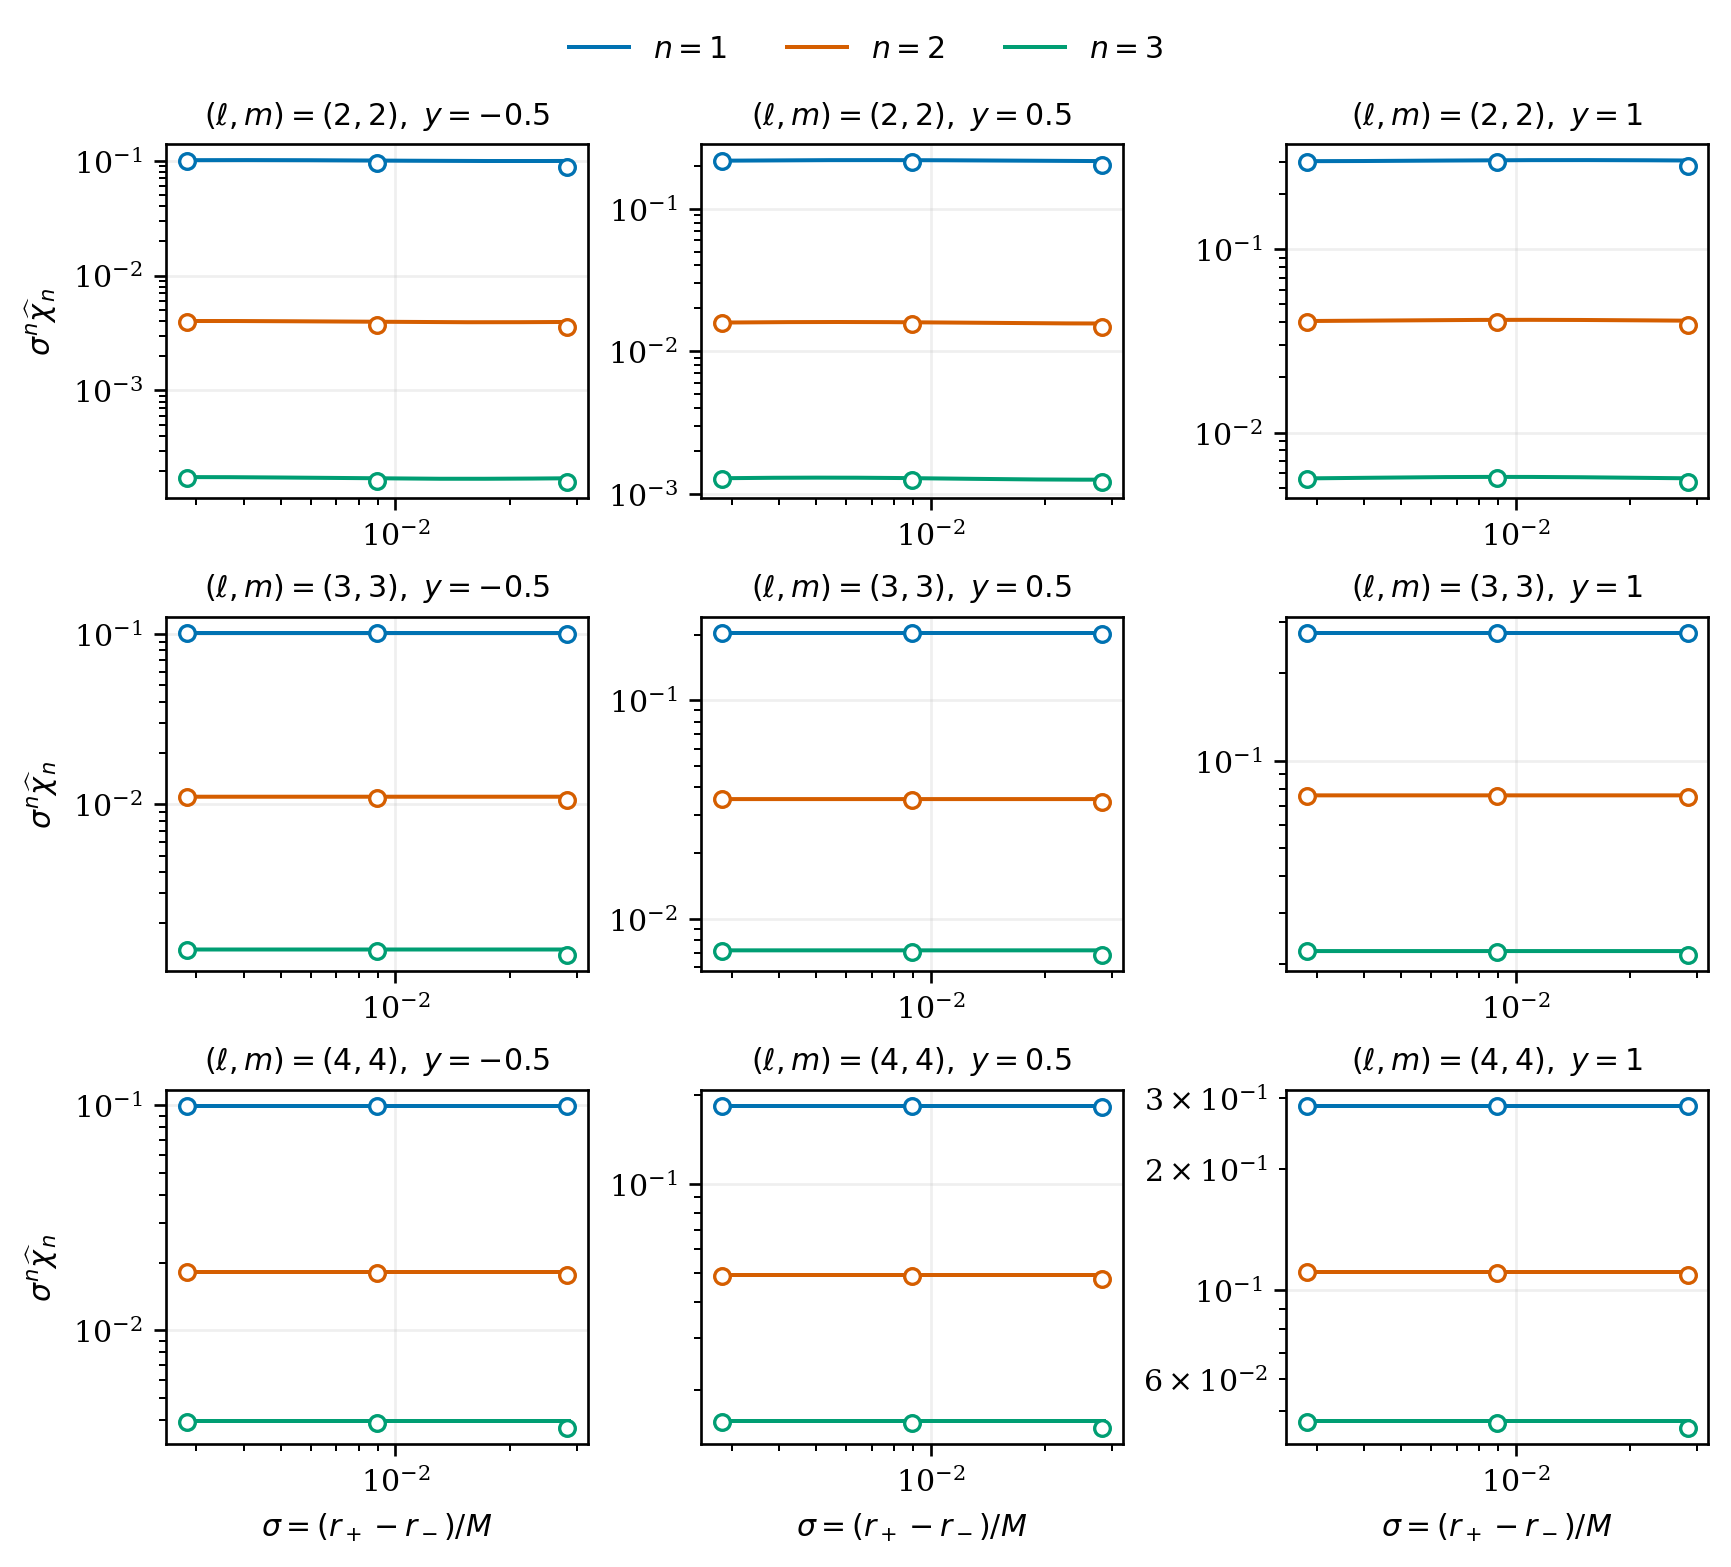
\includegraphics[width=0.96\textwidth]{../../figures/kerr_scalar_principal_expanded_20261014.png}
\caption{Principal-mode response coefficients after removing the predicted
envelope, $\sigma^n\widehat\chi_n$.  Rows are $(2,2),(3,3),(4,4)$ and
columns are $y=-0.5,0.5,1$.  Colors label $n=1,2,3$.  Lines are the
parameter-free analytic functions evaluated at $180$ display locations;
symbols are the independently computed full Kerr spectral points.
Each numerical series has three spins and paired spectral/quadrature
resolutions.  The solid functions retain the two-branch logarithmic phase.
The comparison tests the leading coefficient as well as the envelope power.}
\label{fig:principal-expanded}
\end{figure*}

The acceptance criteria for this large-response experiment combine
paired changes of the real and complex horizon response, spectral tails,
field-dependent off-grid radial residuals and separately recorded flux
interference errors.  Both absolute $|T_n^{(1)}+R_n^{(1)}|$ and relative
$|T_n^{(1)}+R_n^{(1)}|/(|T_n^{(1)}|+|R_n^{(1)}|)$ are retained.
The axisymmetric figures continue to use their original absolute gate.
The principal-response figure uses the local and paired-response criteria
reported with Table~\ref{tab:principal-verification20261014}; the CSV also
identifies which points pass the original absolute gate.
The thresholds are $10^{-5}$ for both paired horizon-response changes,
$10^{-4}$ for the independent quadrature change, $10^{-6}$ for the
off-grid radial residual, $10^{-8}$ for the spectral tail, and $10^{-6}$
for the normalized interference balance.  The original absolute gate is
$10^{-8}$.  These tolerances are applied uniformly across the grid.
The physical flux correction multiplies each coefficient and its absolute
numerical error by $\epsilon_n|{\cal A}_{\rm in}|^{2n}$.

The observed resolution changes quantify numerical error, while the
difference from the parameter-free prediction quantifies the finite-$\sigma$
correction to the leading matched approximation.
The envelope in Eq.~\eqref{eq:principal-law} follows analytically from
the equal real parts of the two principal branches and the convergence of
the nonlinear source integral.  Three-spin slope estimates provide a
finite-window diagnostic; the coefficient comparison supplies the direct
test of the derived response function.
